\chapter{Resultat}
Fra programmet gennemgået i kapitel \ref{chap:program} fås der kun gennemsnittelige ventetider for hvert år skrevet i en tekstfil.
For at kunne sammenlige disse resultater når antallet af landingsbaner ændres, skal programmmet da køres flere gange, hvor værdien \code{runways} ændres.

Programmet \code{plot.py} plotter et histogram med de filer som skrives som et command-line argument.
Med dette program er de to datasæt \code{15Y1K.txt} og \code{15Y2K.txt} (genereret med \code{airplanes.py}) blevet plottet, hvilket kan ses i Figur \ref{fig:results}.

\begin{figure}[h]
	\centering
	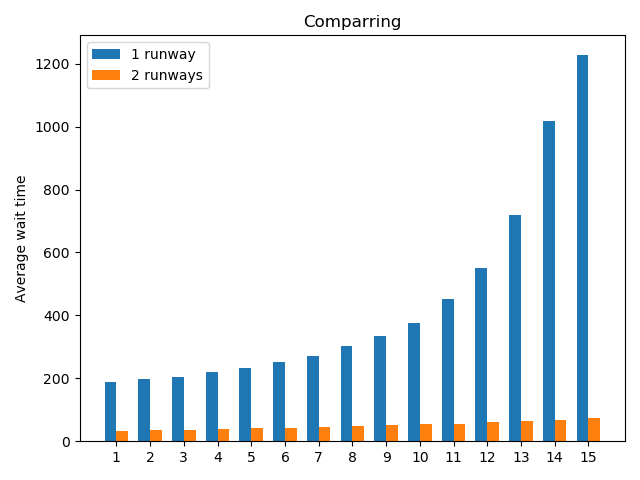
\includegraphics[scale=0.7]{fig/img/results_15Y.png}
	\caption{Et plot over den gennemsnittelige ventetid per fly over 15 år ved både én og to landingsbaner.} \label{fig:results}
\end{figure}

På figuren ses det tydeligt at to landingsbaner er en forbedring på den gennemsnittelige ventetid.
Ventetiden er på omkring 200 sekunder i det første år med én landingsbane, mens den for to er på omkring 30 sekunder.
Det kan også ses at ventetiden med én landingsbane efter mange år begynder at stige meget hurtigt, mens den med to landingsbaner bliver ved med at stige en lille smule i alle 15 år.
Generelt bliver ventetiden mere end fem gange så lille hvis der tilføjes en ekstra landingsbane.

En anbefaling til lufthavnsbestyrelsen må da være at det efter ti år vil blive nødvendigt at udvide landingsfaciliteterne, da flyene i gennemsnit vil komme til at vente omkring $6-7$ minutter med blot én landingsbane.
Dog vil det være en stor fordel for lufthavnen at udvide så hurtigt som muligt, da det altid vil forbedre ventetiden markant, hvilket vil resultere i mere tilfredse kunder.
